%%%%%%%%%%%%%%%%%%%%%%%%%%%%%%%%%%%%%%%%%%%%%%%%%%%%%%%%%%%%%%%%%%%%%%%%%%%
% * <sonya.hanson@choderalab.org> 2015-04-23T18:56:00.248Z:
%
% 
%
% HEADER: DON'T EDIT THIS!
%%%%%%%%%%%%%%%%%%%%%%%%%%%%%%%%%%%%%%%%%%%%%%%%%%%%%%%%%%%%%%%%%%%%%%%%%%%
% ^ <sonya.hanson@choderalab.org> 2015-04-23T18:57:46.938Z.

\documentclass[11pt]{article}

\title{ Advancing predictive physical modeling through focused development of model systems to drive new modeling innovations}

\usepackage[top=0.5in, bottom=0.5in, left=0.5in, right=0.5in]{geometry}
\usepackage{helvet}
\usepackage{url} % hypderref?
\usepackage{graphicx}
\graphicspath{{figures/}} % The figures are in a figures/ subdirectory.
\renewcommand{\familydefault}{\sfdefault}
\pagestyle{empty}
%\pagestyle{plain}
\usepackage{wrapfig}

% Fancy page-width tables
\usepackage{tabularx}

% Use a package for framed boxes
\usepackage{mdframed}

\usepackage[T1]{fontenc}
\usepackage{amssymb}


\usepackage{setspace}
\usepackage{microtype}

\usepackage{amsfonts}
\usepackage{amsmath}

\usepackage{floatrow}

\usepackage[normalem]{ulem} % for nci.bst

\usepackage{sidecap}
\usepackage[abs]{overpic}
\usepackage{wrapfig}

%\usepackage[round,authoryear]{natbib}
\usepackage{cite}
%\setlength{\bibsep}{0.00in}

\usepackage{hyperref}
\hypersetup{colorlinks=true, urlcolor=black, citecolor=black, linkcolor=black}

\newcommand{\doi}[1]{\href{http://dx.doi.org/#1}{doi:#1}}

\newcommand{\ac}[1]{{\sc \lowercase{#1}}}

\renewcommand{\baselinestretch}{.93}
%\renewcommand{\baselinestretch}{.90}
\usepackage{wrapfig} 

\usepackage{bibspacing}
\setlength{\bibspacing}{\baselineskip}


\graphicspath{{figs/}}

\makeatletter

\newcommand{\captionfonts}{\footnotesize}

\makeatletter  % Allow the use of @ in command names
\long\def\@makecaption#1#2{%
  \vskip\abovecaptionskip
  \sbox\@tempboxa{{\captionfonts #1: #2}}%
  \ifdim \wd\@tempboxa >\hsize
    {\captionfonts #1. #2\par}
  \else
    \hbox to\hsize{\hfil\box\@tempboxa\hfil}%
  \fi
  \vskip\belowcaptionskip}      
\makeatother

\renewcommand{\figurename}{{\bf Figure}}

% Page numbering.
%\pagestyle{plain}
%\pagenumbering{arabic}

\setlength{\abovecaptionskip}{-5pt}

\makeatother

\renewcommand{\refname}{Bibliography and References Cited}

\setlength{\parindent}{0pt} % Don't indent first line
%\setlength{\parskip}{1ex plus 0.5ex minus 0.2ex} % Add some space between paragraphs
\setlength{\parskip}{0.8ex} % Add some space between paragraphs

\begin{document}

%======================================
% CITE OUR REFS FIRST
%\phantom{
%\cite{mobley-chodera-dill:2006:jcp:orientation-restraints,mobley-chodera-dill:2007:jctc:confine-and-release,shirts-mobley-chodera-pande:2007:jpcb:dispersion-corrections,chodera:jcp:2007,shirts-mobley-chodera:2007:annu-rep-comput-chem:prime-time,shirts-chodera:jcp:2008:mbar,ncmc,chodera-shirts:jcp:2011:gibbs,chodera:curr-opin-struct-biol:2011:drug-discovery,chodera-shirts:jcamd:2013:yank}
%\cite{gunner:biophys-j:1997:mcce,gunner:bba:2000:proton-electron-transfer,gunner:biophys-j:2002:mcce,gunner:j-comput-chem:2009:mcce2,gunner:jmb:2009:mcce2-hsa,gunner:proteins:2010:reaction-center,dutton:biochem:1994:photosynthetic-reaction-center,gunner:proteins:2010:reaction-center,gunner:photosynth-res:2013:photosynthetic-reaction-center,gunner:bba:2000:proton-electron-transfer,gunner:j-comput-chem:2009:mcce2,nielsen-gunner-garciamoreno:proteins:2011:pka-cooperative,stanton-houk:jctc:2008:benchmarking-pka-prediction}
%}

%%%%%%%%%%%%%%%%%%%%%%%%%%%%%%%%%%%%%%%%%%%%%%%%%%%%%%%%%%%%%%%%%%%%%%%%%%%
% SPECIFIC AIMS
%%%%%%%%%%%%%%%%%%%%%%%%%%%%%%%%%%%%%%%%%%%%%%%%%%%%%%%%%%%%%%%%%%%%%%%%%%%

%{\large \bf SPECIFIC AIMS}

%\eject

%%%%%%%%%%%%%%%%%%%%%%%%%%%%%%%%%%%%%%%%%%%%%%%%%%%%%%%%%%%%%%%%%%%%%%%%%%%
% SIGNIFICANCE
%%%%%%%%%%%%%%%%%%%%%%%%%%%%%%%%%%%%%%%%%%%%%%%%%%%%%%%%%%%%%%%%%%%%%%%%%%%

{\large \bf SIGNIFICANCE}
%2 pages

%Promise of physical methods, how they could transform drug discovery and the design of new small molecules for chemical biology
% (If space permits here we will allude also to how this could help with broader areas too such as engineering of biologics)
Physical methods are poised to transform drug discovery and chemical biology via quantitative, predictive design of small molecules. %Single sentence placeholder for outline

%Limitations of methods and of retrospective tests or application for methods improvements
Unfortunately, these methods still have severe limitations and much work is needed to expand their domain of applicability, but retrospective tests are unsuitable for this. %Single sentence placeholder for outline

%Explain need for blind challenges and how D3R only fills part of need
To truly advance these methods, we need a series of blind challenges focused on pushing the limits of predictive techniques. %Single sentence placeholder for outline

%Discuss importance of SAMPL (including publication/citation count, previous successes in advancing the field, focus), need for funding to:
%   a. Continue SAMPL
%   b. Extend SAMPL to bridge to D3R rather than leaving a ?capability gap? (here?s where I explain why this is distinct from D3R -- this is crucial)
SAMPL has been vital to fulfill this role; here we propose to continue and extend SAMPL via collection of a set of carefully selected experimental data in order to drive further improvements in modeling. %Single sentence placeholder for outline

%Wrap up with how this will realistically help advance binding prediction in a realistic timeframe (a brief mention of CASP will likely be appropriate even though we don?t follow the same model)
This work is necessary in order to advance modeling to the point where it can reliably guide drug discovery efforts, reducing time consuming and costly trial and error. %Single sentence placeholder for outline


{\large \bf INNOVATION}
% 1 page

%SAMPL drives science in our groups and in the field
   %a. Give examples from our groups from prior SAMPLs
   %b. Examples from field in prior SAMPLs
         %b.1 Figure showing progression in hydration free energy accuracy across a couple of SAMPLs or comparing two SAMPLs?
    %c. Mention uniqueness of SAMPL -- there are other predictive challenges (D3R, pKa coop, CASP) but none focused on driving quantitatively predictive protein-ligand modeling
We will discuss how SAMPL has previously driven innovation in the field.


% Innovation in experimental pipelines (Aim 3)
Innovation here will include developing new, high-throughput experiments for studying protein ligand binding (Aim 3).

% Innovative reference calculations (Aim 4)
In Aim 4, we will not only run SAMPL community challenges, but also perform our own reference calculations with the latest techniques, testing their accuracy and using these to assess the current state-of-the-art.

% Innovation in analysis of method performance, comparison of methods, workflow science? (Aim 4)
Innovation here will also involve careful assessment of how to compare methods and analyze their relative performance in a statistically sound way.

{\large \bf APPROACH}
% 9 pages


%Aim 1 - Generate new data for simple SAMPL blind challenges on physical property prediction (1.5 pages)
{\bf Aim 1: Generate new data for ``simple'' SAMPL blind challenges on physical property prediction.}
We will develop new solution-phase datasets for druglike small molecules. These data can test critical aspects of small molecule modeling (including accounting for interactions and treatment of protonation/tautomeric state) and improve our ability to predict physical properties relevant to drug discovery in new regions of chemical space. We will initially focus on distribution between organic phases and on pKa?s and their modulation by solvent environment, using these data to drive improvements in the modeling of ligand interactions.

%Explain what science -- log D/logP, pKa primarily but mention possible other areas of interest
    %Industry partnerships (and past precedent)
%Compare log D accuracy vs hydration accuracy, highlight issues and explain relevance to drug discovery; note lessons learned in SAMPL5

%Aim 2 - Measure binding of novel host-guest complexes for introductory ligand binding challenges (2 pages)
{\bf Aim 2: Measure binding of novel host-guest complexes for introductory ligand binding challenges.}
We will measure new host-guest binding free energies for cucurbiturils and deep-cavity cavitands, yielding further host-guest binding challenges which span between physical property prediction and protein-ligand binding. Host guest systems are some of the simplest cases of molecular recognition, and thus these binding data will drive improvements in modeling of simple binding systems with techniques of relevance to drug discovery.

%Intro lessons learned on HG systems, relevance to drug discovery
%Isaacs science
%Edit to be consistent with Gibb section below -- this uses 3rd person initially.
{\bf Cucubituril derivatives for host-guest binding.} The Isaacs group has previously participated in the SAMPL challenges and supplied unpublished host-guest binding constants~\cite{ma_acyclic_2012-2, cao_absolute_2014, She_she_glycoluril-derived_2016}.  Our participation was quite stimulating for us and influenced our investigation of the biomedical applications of acyclic CB[n]-type receptors (a.k.a Calabadions). Cucurbit[n]uril receptors are particularly well suited for the SAMPL challenges because they exhibit: 1) high binding constants toward suitable guests in water (routinely $\mu$M to nM; occasionally pM to fM)~\cite{cao_attomolar_2014, liu_cucurbituril_2005, mock_structure_1986, assaf_cucurbiturils:_2015, moghaddam_new_2011, shetty_can_2015, biedermann_release_2012}, 2) high selectivities between structurally related guests which translate into large $\Delta \Delta G$ values~\cite{isaacs_stimuli_2014}, 3) low molecular weights (1000-2000 amu) which allows high levels of theory to be used, and 4) limited conformational degrees of freedom.  Herein, we propose to continue to participate in the next three SAMPL challenges during the proposed five year funding period by resynthesizing previously published CB[n]-type receptors of increasing complexity, measure Ka values and determine host-guest stoichiometry and geometry toward biologically relevant guests which will allow the computational chemists to push the boundaries of the free-energy prediction of receptor?ligand complexes.  Figure~\ref{fig:CB} shows the chemical structures of three hosts -- Me4CB[8]~\cite{vinciguerra_synthesis_2015}, glycoluril hexamer~\cite{lucas_templated_2011}, and acyclic CB[n]-type receptors~\cite{ma_acyclic_2012, ma_acyclic_2012-1, zhang_acyclic_2014, gilberg_acyclic_2015, sigwalt_acyclic_2016, zhang_acyclic_2014-1} which span the range from preorganized macrocyclic host to uncharged acyclic but preorganized host to highly charged acyclic host.

\begin{figure}[h]
\begin{centering}
\resizebox{\textwidth}{!}{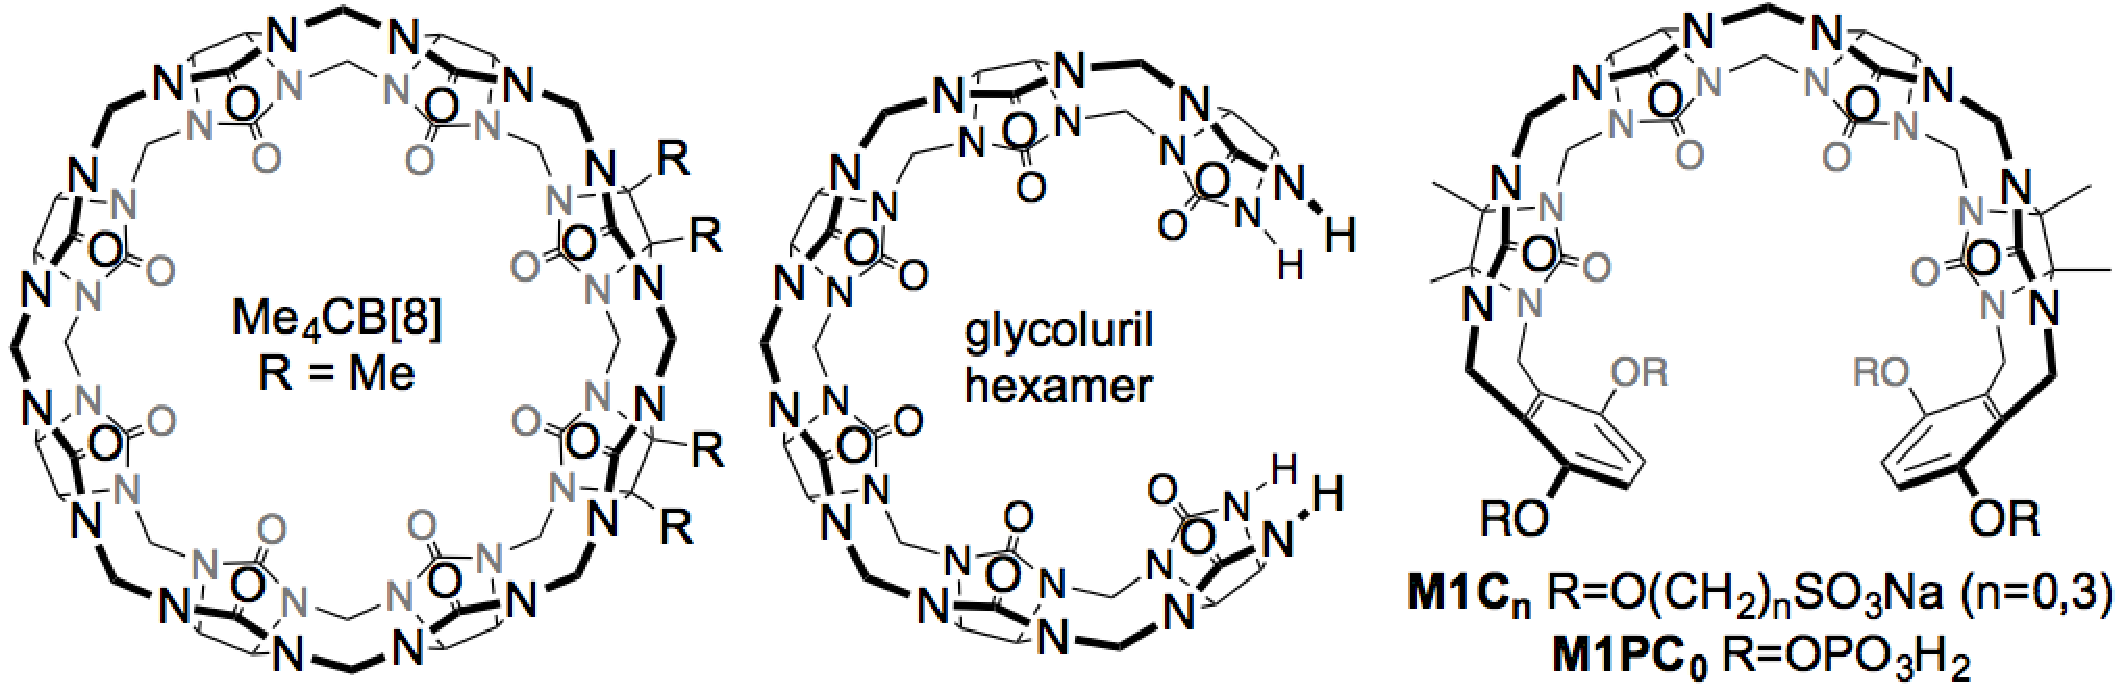
\includegraphics{figures/CB.pdf}}

%\end{centering}
\vspace{0.1in}
\caption{\footnotesize {\bf Structures of Me$_4$CB[8], glycouril hexamer, and acyclic CB[n]-type receptors.}
\label{figure:CB}}
\end{centering}
\end{figure}

\emph{SAMPL6.}  For this challenge we propose to measure $K_a$ and $\Delta H$ values, stoichiometry, and geometry for the interaction of Me4CB[8] (nicely water soluble CB[8] derivative) toward 15 guests (chosen from top selling drugs, Table CB1) by either direct or competition isothermal titration calorimetry (ITC), UV/Vis or fluorescence indicator displacement assay, or NMR competition experiments which we are very experienced with~\cite{cao_attomolar_2014, liu_cucurbituril_2005, ma_acyclic_2010, she_glycoluril-derived_2016}.  Our selection of Me$_4$CB[8] and top 100 drugs was based on a desire to increase the level of complexity of the computational challenge by: 1) changing host flexibility (e.g. Me$_4$CB[8] can exhibit ellipsoidal deformation)~\cite{vinciguerra_synthesis_2015}, 2) by allowing the possibility of binary or ternary (e.g. 1:1 and/or 1:2 host:guest) complexes~\cite{ko_supramolecular_2007, barrow_cucurbituril-based_2015, urbach_molecular_2011}, 3) using drugs with several potential binding epitopes to include sampling issues.  Host:guest stoichiometry and geometry (e.g. which binding epitope is complexed) will be addressed by ITC ``n'' values, Job plots monitored by UV/Vis or NMR~\cite{connors_binding_1987}, and by 1H NMR complexation induced changes in chemical shifts~\cite{masson_cucurbituril_2012}.  All three sets of studies will be conducted in phosphate buffered saline (pH 7.4 with physiological salt) which introduces further complexity due to competitive interaction between the C=O portals of CB[n]-type receptors and metal ions via ion-dipole interactions which reduces the observed Ka values~\cite{marquez_mechanism_2004}.

\begin{wraptable}{l}{7.5cm}
\begin{tabular}{l | l}
{\bf drug} & {\bf features} \\
\hline
memantine & adamantane; 1:1 \\
saxagliptin & adamantane; 1:1 \\
premarin & steroid \\
pancuronium & steroid\\
varenicline & 1:1 vs 1:2 \\
valsartan & pKa 4.37 \\ 
omeprazole & pKa 4.77 \\
ranolazine & pKa 7.17; epitopes \\
pradaxa & pKa 3.87; epitopes \\
nilotinib & epitopes; pKa 6.3 \\
sensipar & epitopes; folding \\
vyvance & diamine; epitopes; folding \\
minocycline & tetracyclin; amino aniline \\
\end{tabular}
\caption{\label{table:CB} Selected drugs as guests }
\end{wraptable}

\emph{SAMPL8.} We propose to study host:guest complexes of glycoluril hexamer toward the 15 drugs (Figure CB1).  We select glycoluril hexamer for this challenge because it: 1) increases the conformational dynamics of the host, and 2) influences the number and energy of solvating (and unusually coordinated) water molecules that are implicated in the observed high binding constants for CB[n]-guest complexes~\cite{biedermann_release_2012, biedermann_hydrophobic_2014}.  Furthermore, in selecting the drugs, we have chosen several that have pKa values in the 3.8 to 7.4 range.  Similar to biomolecular host-guest systems, CB[n]-type receptors are well known to induce pKa shifts (up to 4 pKa units) of complexed guests~\cite{saleh_activation_2008, nau_deep_2011, ghosh_strategic_2012}, and the ability of computation to replicate and predict such shifts and their impact on Ka are of high significance.
 
\emph{SAMPL10} We will focus on acyclic CB[n]-type receptors (e.g. M1C$_3$, M1C$_0$, and M1PC$_0$ that contain anionic solubilizing groups attached via different linker lengths.  As in SAMPL2, these acyclic CB[n]-type receptor introduces conformational complexity and influences the free energy of the solvating H$_2$O molecules in the free host.  Moreover, the presence of 4 anionic groups in close proximity to the cavity are expected to have a significant influence on the balance between ion-dipole interactions and the solvation of the free host.

%Gibb science

%CHODERA FEEDBACK TO INCORPORATE HERE:
%* We need to emphasize why the octa-acid system has proven to be so valuable for modelers in the introduction: What specific physical challenges does the system probe, and what have we learned? We also need to add citations to the meta-analysis and maybe even all of the papers that addressed this system. David can likely address this.
%* I'm a bit concerned that proposing to measure only five ligands per compound is going to be perceived as lacking in statistical power required to assess accuracy, and that this specific aspect will be a liability. Is it possible to do more than that, or would this require a significantly larger chunk of money or access to automated ITC technology? Alternatively, we can be vague about how many compounds we will use or focus on the total number of compounds across all hosts. (DLM: I should probably recast a bit somewhere to explain how much we'll learn across hosts.)

{\bf Gibb deep cavity cavitands for host-guest studies.} 
During SAMPL4~\cite{gibb_binding_2013} and SAMPL5~\cite{sullivan_binding_2016} we focused on two hosts: the octa-acid 1 (R = H) and another octa-acid derivative with four methyl groups positioned at the portal of the binding pocket (1, R = Me).  These studies used Isothermal Titration Calorimetry (ITC) to measure the thermodynamics of respectively: 1 (R = H) complexing a range of carboxylate guests, and the binding of carboxylate and trimethylammonium guests to both hosts (1, H = H and Me).  In both cases NMR was also used in a confirmatory role for free energy data.  SAMPL5 emphasized that slight differences in the shape of the hydrophobic pocket of the host can in the case of some guests have a profound affect on affinity.

\begin{figure}[h]
\begin{centering}
\resizebox{\textwidth}{!}{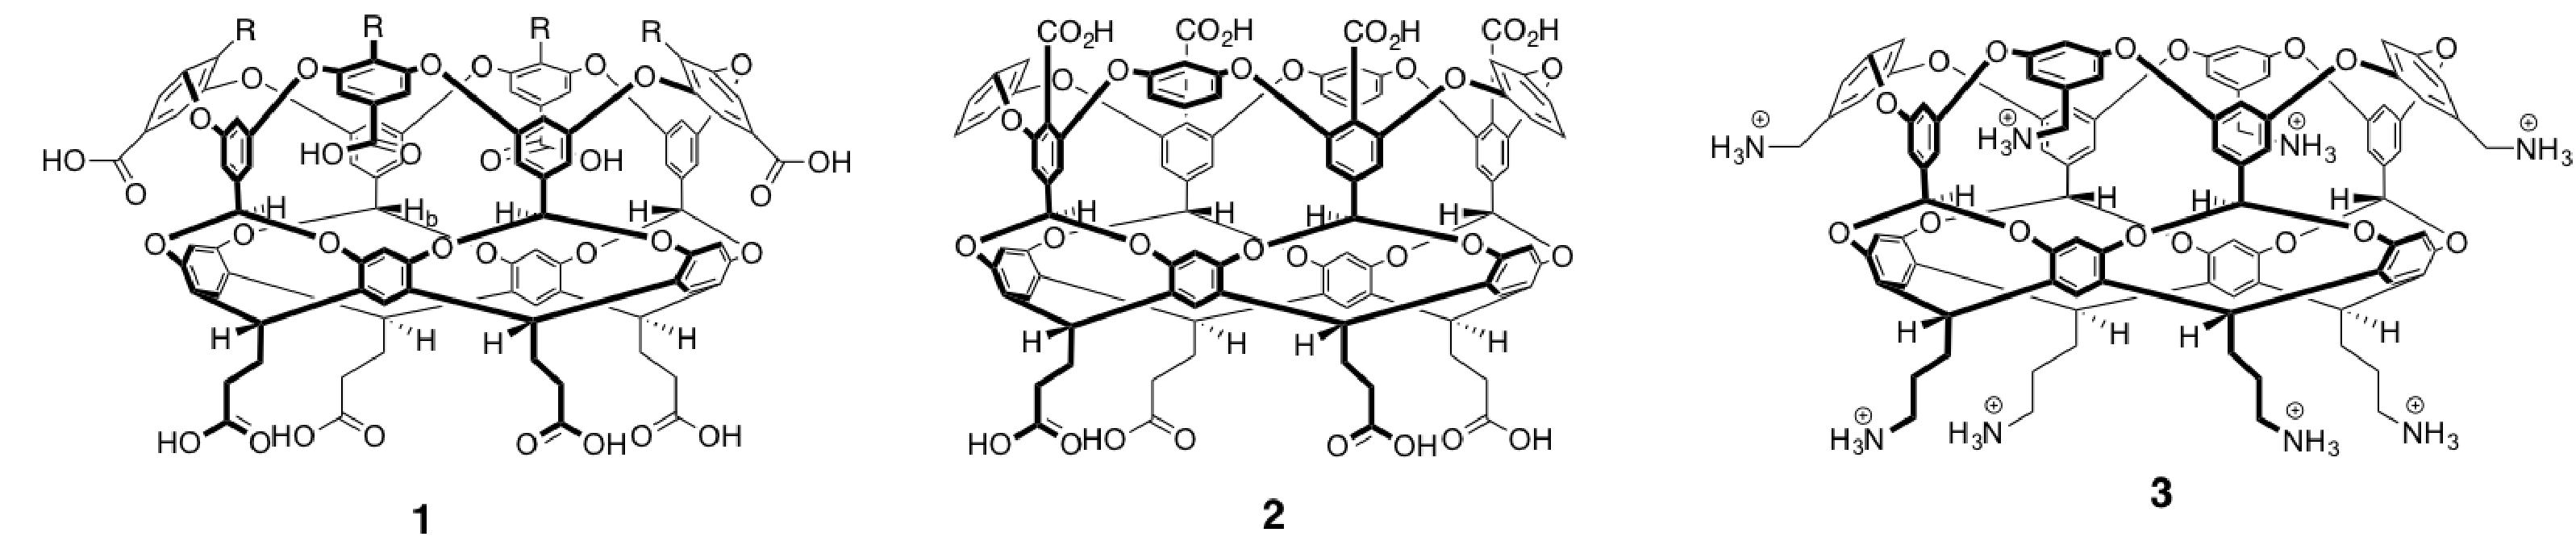
\includegraphics{figures/gdccs.pdf}}

%\end{centering}
\vspace{0.1in}
\caption{\footnotesize {\bf Gibb deep cavity cavitands for SAMPL6-10.}
\label{figure:gdccs}}
\end{centering}
\end{figure}


To continue with this work we will expand on the range of hosts by including 2 and 3 in our ITC studies.  Like cavitand 1, host 2 is an octa-acid derivative.  However, the four benzoate groups are relocated from the extreme exterior in the case of 1, to the rim of the binding pocket in 2.  We surmise that this will have a direct effect on the binding of charged guests, but more subtly, an indirect effect on guest complexation via changes to the solvation of the empty host.  Octa-trimethylammonuim cavitand (``positand'' 3) has the same overall architecture as host 1, but inverts the charges on the water solubilizing exterior coat.  It is not entirely clear at this juncture if this switch in groups relatively remote from the pocket can directly affect guest complexation.  However related (unpublished) results suggest that it can.

Guests for the five proposed ITC studies will be obtained from commercial sources and will be selected on both the limitations of force-fields available to the computationalists and new data as it is gathered.   

SAMPL6 will involve hosts 1 and 2 with a set of five, previously uninvestigated guests.  The principal aim for our group will be to examine how the location of the carboxylate affects guest binding.  Building on what the computational chemists learn from this study, SAMPL7 will compare hosts 1 and 3 with a different set of five guests.  We anticipate that because of the relative remoteness of the charged groups in these two hosts, the effects of switching charges will be subtler than the differences between 1 and 2.  SAMPL8 will switch gears and consider the effects salts have on guest binding.  Thus, we will compare the effects of NaCl and NaI on the complexation of five guests to 1.  We have previously shown that iodide has a weak affinity for the binding pocket of 1, whilst sodium ions have an affinity for the outer carboxylates~\cite{carnegie_anion_2014}, and this will be made clear to the participants.  We will follow on from this with SAMPL9 looking at the affects of these same two salts on the complexation of five guests to 3.  We have not yet quantified the complexation of this salt to host 3, but expect the iodide to have affinity for both the pocket and the positively charged solubilizing groups.  Finally, for SAMPL10 we will consider the effects of co-solvents on the binding of five guests to 1 and 2.  This is for us an entirely new area, but we expect binding to be weaker because of co-solvent affinity for the binding pocket leading to competition; there will be an apparent weakening of the hydrophobic effect.  However, the precise nature of this weakening phenomenon are unclear.


%Aim 3 - Generate biologically relevant advanced model systems for protein-ligand binding challenges. (2 pages) 
{\bf Aim 3. Generate biologically relevant advanced model systems for protein-ligand binding challenges.}
We will identify suitable biological protein-ligand model systems (difficult but tractable in order to push the limits of physical techniques) then measure binding and develop these for blind challenges. This will include binding studies on human serum albumin and bromodomains or aspartyl proteases; initial binding data will be expanded by the selection of additional ligands or the creation of mutations in the protein that modulate binding.


%Aim 4 - Coordinate, run, and analyze blind challenges to advance modeling of binding (1.5 pages)
{\bf Aim 4. Coordinate, run, and analyze blind challenges to advance modeling of binding.}
The data collected in Aims 1-3 will drive annual SAMPL blind challenges, allowing the field to test the latest methods and force fields to assess progress, compare them against one another head-to-head, and perform sensitivity analysis to learn how much different factors (protonation state, tautomer selection, solvent model, force field, sampling method, etc.) affect predictive power. Results will then feed back into improved treatment of these factors for subsequent challenges, driving regular cycles of application, learning, and advancement.
%Coordinate and run SAMPL blind challenges
	%Run reference calculations to:
		%a. Test current standard methods/FF
		%b. Facilitate others learning (swap method or FF)
		%c. Do sensitivity analysis (learn what?s important)
		%d. (Give examples of what we?ve learned from this)
		%e. (We will make inputs, outputs, and methods available too)
	%Select and announce null models, run them
	%Do statistical analysis of results (& compare to nulls), report back
	%Work with D3R on meeting coordination
	%Coordinate follow-up experiments as needed (cite examples when this was desirable)
	%Coordinate with JCAMD on special issues
	%Data archival and dissemination
	%D3R coordination:
	%	a. Co-running workshops with D3R
	%     b. Coordinating challenges with them, submission deadlines offset from D3R challenges



%%%%%%%%%%%%%%%%%%%%%%%%%%%%%%%%%%%%%%%%%%%%%%%%%%%%%%%%%%%%%%%%%%%%%%%%%%%%%%%%%%%%%%%%%%%%%%%%%%%%%%
% TIMELINE
%%%%%%%%%%%%%%%%%%%%%%%%%%%%%%%%%%%%%%%%%%%%%%%%%%%%%%%%%%%%%%%%%%%%%%%%%%%%%%%%%%%%%%%%%%%%%%%%%%%%%%

{\bf \large TIMELINE} %1 page minus a paragraph
%"The timeline is actually likely to be very important here, so I'd strongly suggest we include it, if not expand it to one full page. We have to "sell" the reviewers on how the concept would play out into actual challenges, advances, etc. so that they get a concrete idea of all the good things that will come of this. We should mention when we would hold blind challenges, when data would be released, when meetings would occur, when benchmarks would be published, and what datasets would be generated for the community."



%%%%%%%%%%%%%%%%%%%%%%%%%%%%%%%%%%%%%%%%%%%%%%%%%%%%%%%%%%%%%%%%%%%%%%%%%%%%%%%%
% FIGURE: AIMS OVERVIEW
%%%%%%%%%%%%%%%%%%%%%%%%%%%%%%%%%%%%%%%%%%%%%%%%%%%%%%%%%%%%%%%%%%%%%%%%%%%%%%%%
%\begin{figure}[h]
%\begin{centering}
%\resizebox{\textwidth}{!}{\includegraphics{figures/timeline.pdf}}

%\end{centering}
%\vspace{0.1in}
%\caption{\footnotesize {\bf Timeline.}
%\label{figure:aims-overview}}
%\end{figure}
%%%%%%%%%%%%%%%%%%%%%%%%%%%%%%%%%%%%%%%%%%%%%%%%%%%%%%%%%%%%%%%%%%%%%%%%%%%%%%%%

%%%%%%%%%%%%%%%%%%%%%%%%%%%%%%%%%%%%%%%%%%%%%%%%%%%%%%%%%%%%%%%%%%%%%%%%%%%%%%%%%%%%%%%%%%%%%%%%%%%%%%
% COLLABORATION MANAGEMENT PLAN
%%%%%%%%%%%%%%%%%%%%%%%%%%%%%%%%%%%%%%%%%%%%%%%%%%%%%%%%%%%%%%%%%%%%%%%%%%%%%%%%%%%%%%%%%%%%%%%%%%%%%%

{\large \bf COLLABORATION MANAGEMENT PLAN} % 1 paragraph


{\large \bf OUTLOOK} %or conclusions. 0.5 page


%%%%%%%%%%%%%%%%%%%%%%%%%%%%%%%%%%%%%%%%%%%%%%%%%%%%%%%%%%%%%%%%%%%%%%%%%%%%%%%%%%%%%%%%%%%%%%%%%%%%%%
% BIBLIOGRAPHY
%%%%%%%%%%%%%%%%%%%%%%%%%%%%%%%%%%%%%%%%%%%%%%%%%%%%%%%%%%%%%%%%%%%%%%%%%%%%%%%%%%%%%%%%%%%%%%%%%%%%%%

\eject

%\footnotesize
%\scriptsize
%\bibliographystyle{acm}
\bibliographystyle{nci}
%\bibliographystyle{nar}
\bibliography{sampl-r01}

\end{document}